\chapter{Measured Data}
\label{app:gatheredData}
\newpage
\begin{figure}[H]
	\centering
	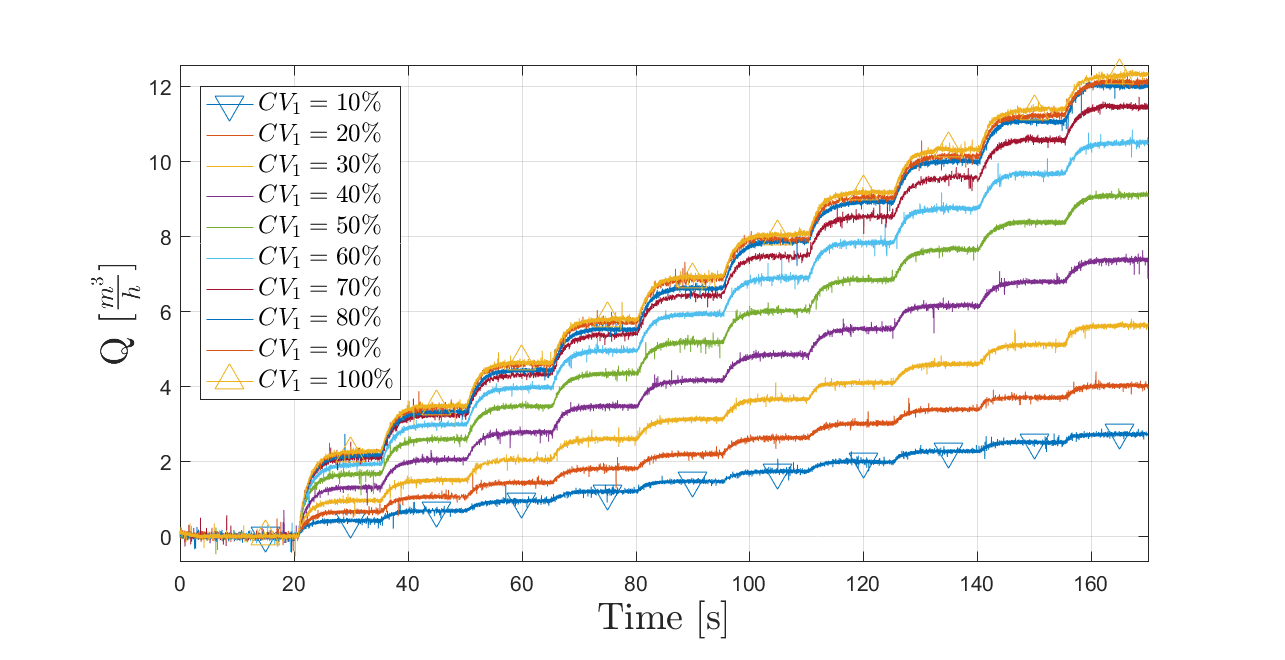
\includegraphics[height=\textwidth, width=\textheight, keepaspectratio, angle=270]{figures/05mathematicalModelling/measuredFlow.eps}
	\caption{Measured Flow}
\end{figure}

\begin{figure}[H]
	\centering
	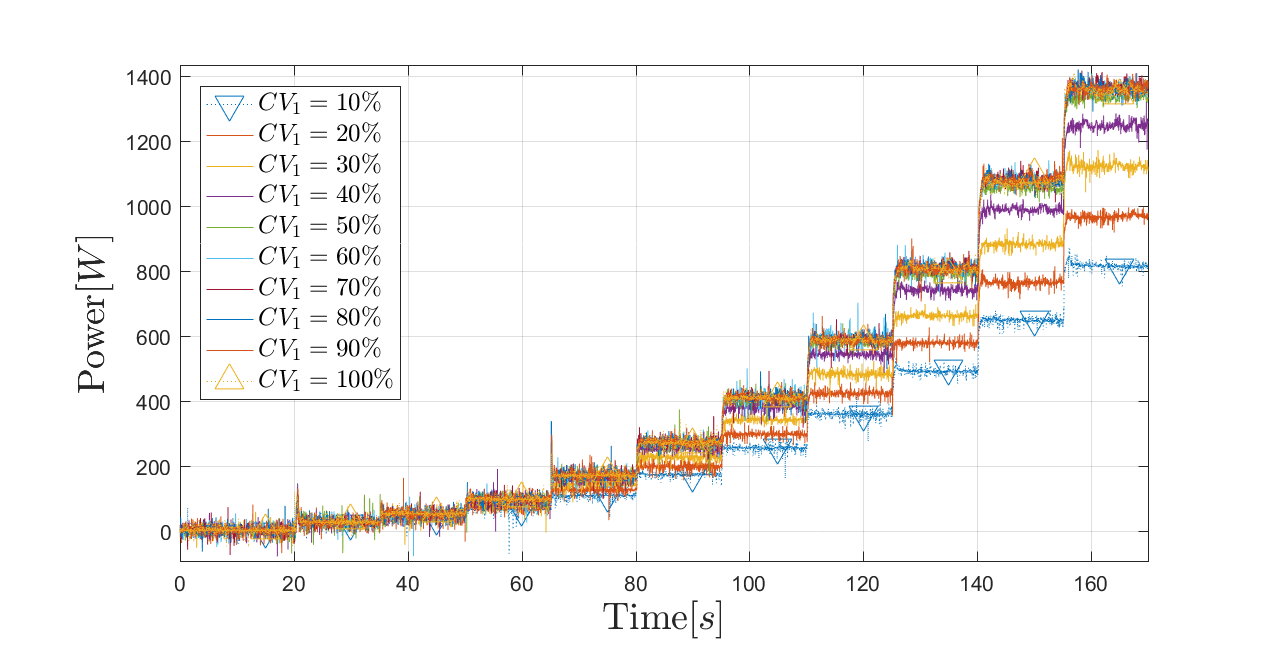
\includegraphics[height=\textwidth, width=\textheight, keepaspectratio, angle=270]{figures/05mathematicalModelling/measuredPower.eps}
	\caption{Measured Power}
\end{figure}

\begin{figure}[H]
	\centering
	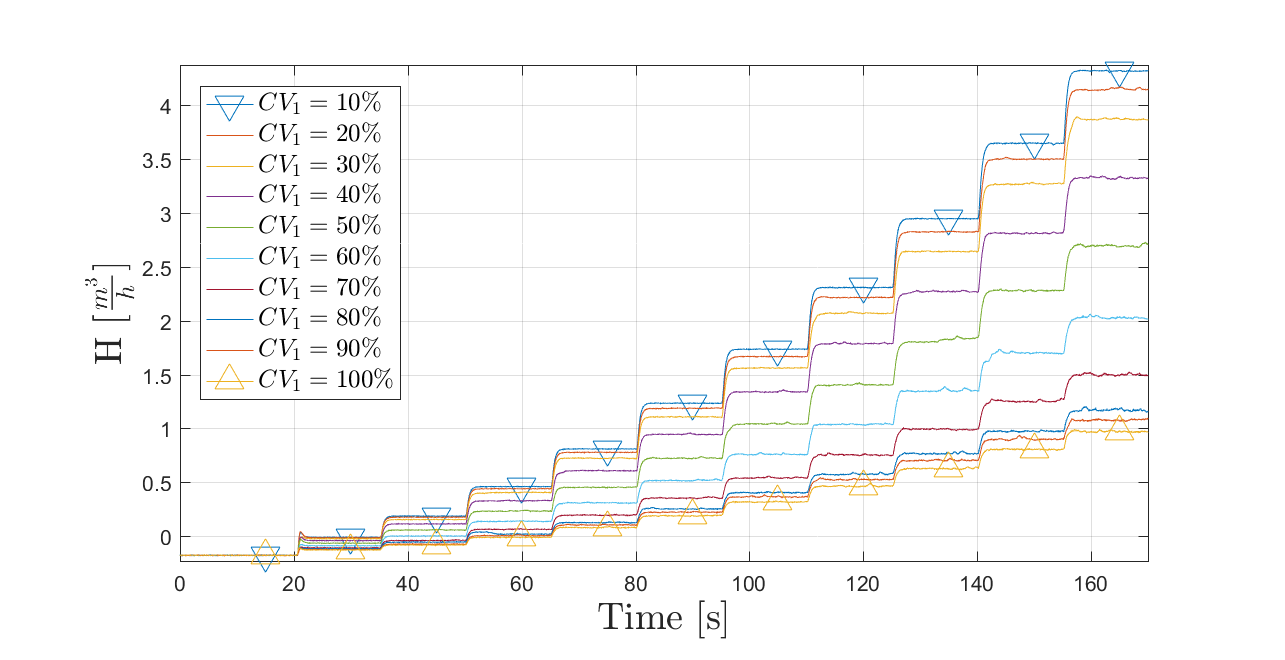
\includegraphics[height=\textwidth, width=\textheight, keepaspectratio, angle=270]{figures/05mathematicalModelling/measuredPressure.eps}
	\caption{Measured Pressure}
\end{figure}

\begin{figure}[H]
	\centering
	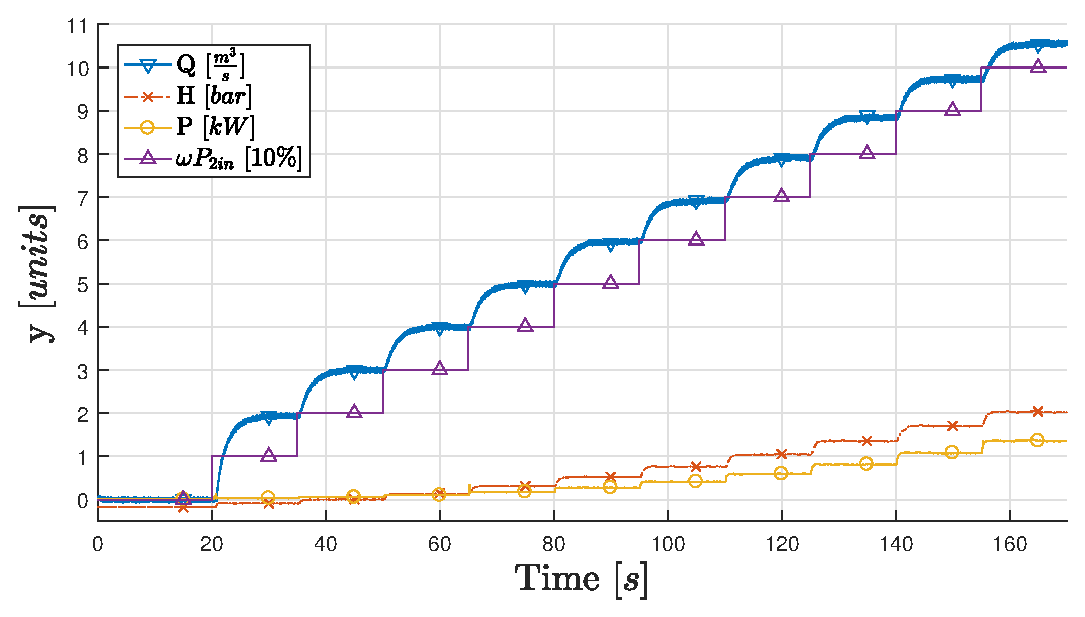
\includegraphics[height=\textwidth, width=\textheight, keepaspectratio, angle=270]{figures/04ExperimentsAndLabWork/testrun.eps}
	\caption{$Q$, $H$, $P$ and stair input $\omega P_{2in}$ at $CV_1 = 70\%$}
\end{figure}